%% ==============================
\chapter{\iflanguage{ngerman}{Ergebnisse}{Results}}
\label{sec:results}
%% ==============================
\section{Hardware and Setup for the Evaluation}\label{c6_sec_setup_all}
\subsection{Hardware}
The evaluation was conducted on real hardware. For the evaluation, multiple computers as well as multiple robots were used. In the following, a short overview of the used computers, robots and network is given. The different setups used for the evaluation are explained and the placement of the robots during the experiments is shown. 

\subsubsection{Computers}
\begin{wrapfigure}{r}{6cm}
\includegraphics[width=6cm]{Figures/c6/network_setup.pdf}
\caption{Schematic overview of the network setup.} \label{c6_fig_network}
\end{wrapfigure}
The used computers were three off-the-shelf laptops. They are not specially designed for control or real-time tasks. A detailed overview of the exact hardware specifications of the used laptops is shown in Table \ref{c3_tab_pc_overview}. 
It includes the processor and network card, as well as the size of the RAM and what type of RAM was used. The first computer (PC1) is a Tuxedo Polaris AMD Gen3. The second one (PC2) a Lenovo Legion 5 15ACH6H and the third computer (PC3) a Lenovo Legion 5 Pro 16ARH7H.\newline
The setup on the laptops themselves was the same for all of them. A fresh Kubuntu 22.04 was installed. The real-time kernel path PREEMPT\_RT was installed via the Ubuntu "\texttt{pro}" command. Rolling was chosen as the \gls{ros2} distribution. The commit hash, the changes to the \gls{r2c} and the \textit{ros2\_controllers} repositories are based on, is listed in the \autoref{c3_tab_pc_overview}.
% Network card : lshw command
% cpu : lscpu
% memory: sudo dmidecode --type 17
% 1 -> arbeitslaptop
% 2 -> mein laptop
% 3 -> yaxin laptop

\subsubsection{Network}\label{c6_sec_network}
The network switch used in the experiments is a five port switch by NETGEAR. The model is called Prosafe Plus Switch (GS105Ev2). For the evaluation, a separate network was set up. The robots and computers were connected over the switch, as shown in \autoref{c6_fig_network}. The computers were not connected to other networks at the time of the tests. Apart from the traffic caused by the tests, nothing else was routed over the network.



\subsubsection{Robots and Industrial Robot Controllers}\label{c3_sec_used_robots}
The used robots for the evaluation were two industrial robots of the type KUKA KR 3 R540 \cite{noauthor_agile_nodate, noauthor_kuka_kr_3_agiluspdf_nodate}. One robot is depicted in \autoref{ca_fig_r2c_mr_is} on the left site. The robots are a 6-axis jointed-arm robots. They have a maximum reach of $541$ \si{\milli\meter} and a pose repeatability of about $\pm 20$ \si{\micro\meter}. The robots are embedded in the \textit{ready2\_educate} as shown on the right site in \autoref{c3_fig_r2c_mr_is}. On the flange a pneumatic actuated Zimmer gp406 gripper is mounted. The mount is probably specifically designed for the \textit{ready2\_educate} platform, but unfortunately a CAD model for the mount could not be found. This would have been useful, ass the gripper is tilted forward, but the precise angle of the tilt is unknown. \newline
The joint naming convention was followed, meaning the joints are numbered in ascending alphanumeric order starting from the base (joint A1 or joint\_a1) to the flange joint (joint A6 or joint\_a6).\newline
The robot controller utilized in the platform is a KUKA KR C4 compact. The \acrfull{rsi}  was used for communication with the robot controller. The robot controller then converts the commands received via the \gls{rsi} into control commands for the robot.
\begin{table}[H]
    \centering
\begin{tabular}{ |c|c|c|c| }
\hline
\multicolumn{4}{|c|}{Overview of the different computers used during the evaluation} \\
\hline
& PC1 & PC2 & PC3  \\
\hline
\hline
\textbf{Hardware} &  &  & \\\hline
    Processor &
        \begin{minipage}{3.7cm}
	       \vspace{8pt}
		      16 $\times$ AMD Ryzen 7 5800H with Radeon Graphics
	       \vspace{8pt}
	    \end{minipage} & 
        \begin{minipage}{3.7cm}
    	    \vspace{8pt}
    		   12 $\times$ AMD Ryzen 5 5600H with Radeon Graphics
    	    \vspace{8pt}
	    \end{minipage} & 
        \begin{minipage}{3.7cm}
	       \vspace{8pt}
		      16 $\times$ AMD Ryzen 7 6800H with Radeon Graphics
	       \vspace{8pt}
	    \end{minipage} \\\hline
    RAM &
        \begin{minipage}{3.7cm}
	       \vspace{8pt}
		      2 $\times$ 32GB DDR4 Samsung SODIMM 3200 MT/s
	       \vspace{8pt}
	    \end{minipage} & 
        \begin{minipage}{3.7cm}
    	    \vspace{8pt}
    		   2 $\times$ 16GB DDR4 SODIMM 3200 MT/s
    	    \vspace{8pt}
	    \end{minipage} & 
        \begin{minipage}{3.7cm}
	       \vspace{8pt}
		      2 $\times$ 16GB DDR5 SODIMM 4800 MT/s
	       \vspace{8pt}
	    \end{minipage} \\\hline
    Network Card &
        \begin{minipage}{3.7cm}
	       \vspace{8pt}
		      Realtek Semiconductor Co., LtdRTL8125 2.5GbE Controller 1Git/s
	       \vspace{8pt}
	    \end{minipage} & 
        \begin{minipage}{3.7cm}
    	   \vspace{8pt}
    		Realtek Semiconductor Co., RTL8111/ 8168/8411 PCI Express 1Gbit/s
    	   \vspace{8pt}
	    \end{minipage} & 
        \begin{minipage}{3.7cm}
          \vspace{8pt}
		      Realtek Semiconductor Co., RTL8111/ 8168/8411 PCI Express 1Gbit/s
	       \vspace{8pt}
	    \end{minipage} \\\hline\hline
\textbf{Setup} & & & \\\hline
    Operating System & Kubuntu 22.04 &  Kubuntu 22.04 & Kubuntu 22.04 \\\hline
    Kernel & 5.15.0-1039-realtime & 5.15.0-1039-realtime & 5.15.0-1039-realtime  \\\hline
    Real-time Kernel & PREEMPT\_RT & PREEMPT\_RT & PREEMPT\_RT \\\hline
    ROS version & Rolling & Rolling & Rolling \\\hline
        \begin{minipage}{3cm}
        \vskip 4pt
    		   ros2\_control based on commit:\vspace{8pt}
	    \end{minipage} & 0eb319ea43b78b886a & 0eb319ea43b78b886a & 0eb319ea43b78b886a \\\hline
            \begin{minipage}{3cm}
        \vskip 4pt
    		   ros2\_controllers based on commit:\vspace{8pt}
	    \end{minipage} & 05d7a5ec73a02eab2c & 05d7a5ec73a02eab2c & 05d7a5ec73a02eab2c \\\hline
\end{tabular}
    \caption{Three different computers were used for the evaluation. This table presents a detailed overview of the used hardware, as well as the setup on each of the computers.}
    \label{c3_tab_pc_overview}
\end{table}

\subsection{Description of the Test Setup}\label{c6_sec_description}
The fundamental idea for the evaluation was to couple the two robots at the end effector with a distance sensor. Then the robots were moved simultaneous. The executed trajectories were chosen in such a way that the relative pose of the effector's tool center point to each other should stay the same during the execution of the trajectories. Ideally, the measured distance should not change if the robots move simultaneous. This way, the values measured and used for the evaluation were collected from outside the system. \newline
From the measured distance change during the execution of the robots, some performance measures were derived. The resulting performance metric were simultaneousness of the executed movement and the jitter measured during the execution. This allowed for evaluation of the implemented concept regarding those performance metrics. Further, the impact of different \glspl{rmw} on the jitter and simultaneousness was investigated. \newline
\begin{wrapfigure}{r}{8cm}
\includegraphics[width=8cm]{Figures/c6/schematic_messurement_rotation.pdf}
\caption{Mounting of the distance sensor on the gripper. 1A and 1B gripper housing of the first and the second robot. 2 plate with an inclination. 3 the laser of the distance sensor. 4A and 4B exemplary rotation around the aligned axes of rotation of joint\_a6 of the robots. 5 Aligned axes A6.} \label{c6_fig_schematic_gripper_mounting}
\end{wrapfigure}
The utilized distance sensor was a OD1-B035 Mini Pro from Sick. The sensor has a measuring range of $35\pm15$ \si{\milli\meter} and a resolution of $6$ \si{\micro\meter} with a repeatability of $9$ \si{\micro\meter}. Since the measuring range of the distance sensor is very limited, the two \textit{ready2\_educate} platforms were placed front to front as shown in \autoref{c6_fig_robot_placement}. A start configuration, where the arms were fully extended to the front, was chosen (joint\_ai = 0.0, $i \in\{1,6\}$). Then it was tried to align the axis of rotation of joint\_a6 as precise as possible. The distance sensor was mounted on one gripper as shown in \autoref{c6_fig_schematic_gripper_mounting}.\newline
One problem was that the grippers could not be disassembled from the flange. As a solution, a bracket for the distance sensor, which could be firmly gripped by the gripper, was created. The distance sensor was then mounted on the bracket and the bracket fixated by the gripper. On the other gripper a plate was mounted. The plate itself was screwed with on a cuboid. The cuboid was in turn gripped by the second gripper. This is shown as number 2 in \autoref{c6_fig_schematic_gripper_mounting}. The distance between the plate and the distance sensor was measured during the whole execution time.

\paragraph{Quality of Service Profiles}
Two different \gls{qos} profiles were compared, as well as three different \glspl{rmw}. An overview of the most important policy settings utilized in the \gls{qos} profiles are shown in \autoref{c6_tab_reliable_qos} and \autoref{c6_tab_sensor_qos}. For the reliable profile, the reliability was set to RELIABLE in order to guarantee to deliver the sent message. For the sensor profile, the reliability was set to BEST\_EFFORT, meaning that no guarantee is given that the sample is delivered and can potentially even can get lost. The size of the queue was set to five samples. 
\begin{figure}[H]
	\centering
	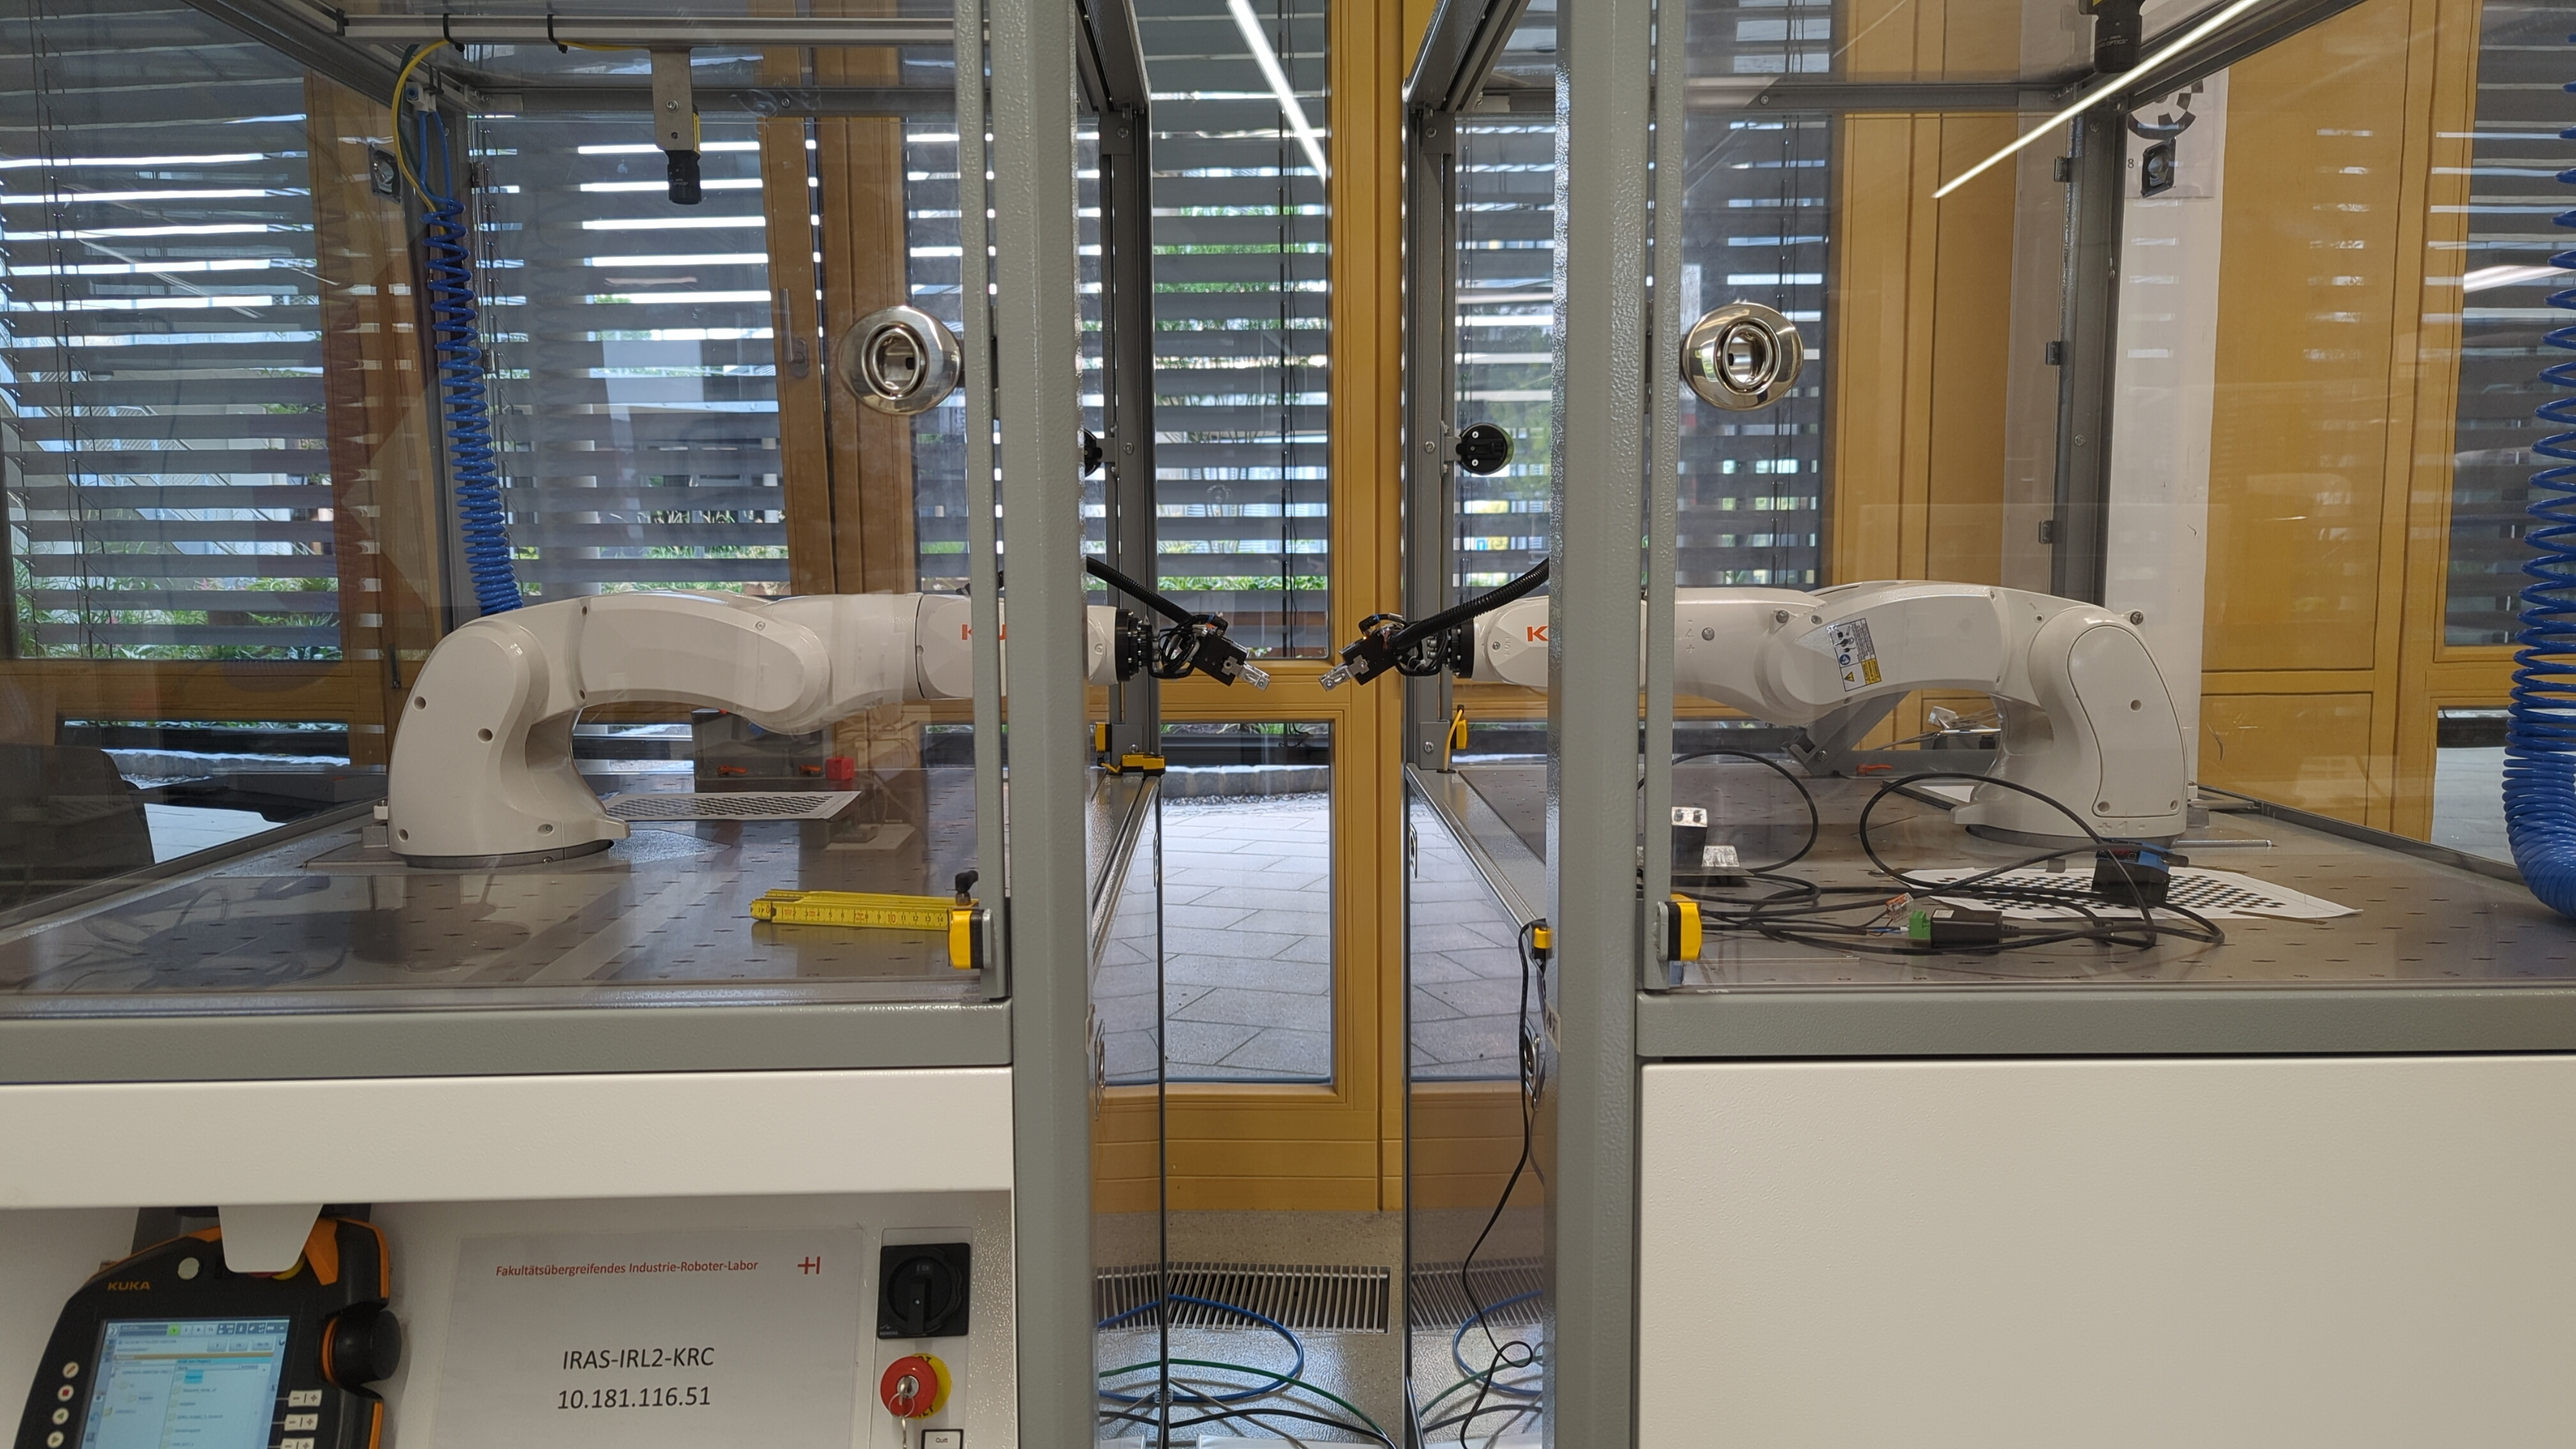
\includegraphics[width=1\textwidth]{Figures/c6/robot_placement.jpg}
	\caption{Placement of the two \textit{ready2\_educate} platforms relative to each other. The two robots are fully extended to be as close as possible to each other. }
	\label{c6_fig_robot_placement}
\end{figure}
\paragraph{Evaluation Overview} In \autoref{c6_tab_evaluation_orverview} an overview of the different tests is given. It is shown which scenario with which \gls{qos} profile and which \glspl{rmw} were combined. As can be seen, scenario 1 was evaluated with each of the three different \glspl{rmw}. For each of the \gls{rmw} the sensor profile and the reliable profile was evaluated. This was done since in this scenario a lot of messages are sent over the network per rotation. The second scenario was only evaluated with one profile, since only two the trajectory message is sent over the network. An in depth explanation of different scenarios as well as the evaluation results and interpretation is given in the following sections.
\begin{table}[H]
    \centering
\begin{tabular}{ |c|c|c|c| }
\hline
\multicolumn{4}{|c|}{Evaluation overview} \\
\hline
& eProsima Fast DDS & Eclipse Cyclone DDS & RTI Connext DDS  \\
\hline
\hline
\textbf{Scenario 1} &  &  &  \\\hline
    Sensor Profile & \checkmark & \checkmark &  \checkmark  \\\hline
    Reliable Profile& \checkmark & \checkmark &  \checkmark  \\\hline\hline
\textbf{Scenario 2} &  &  &  \\\hline
    Sensor Profile & \checkmark & \checkmark &  \checkmark  \\\hline
    Reliable Profile&  &  &    \\\hline
\end{tabular}
    \caption{Overview of which scenarios, \gls{rmw} and \gls{qos} profiles were combined for the evaluation of the concept.}
    \label{c6_tab_evaluation_orverview}
\end{table}
\paragraph{Used Metrics}
In the following, $Q_1$ describes the first quartile or 25th percentile and $Q_3$ are the third quartile or 75th percentile. Outliers are data points, with a value $v$, where $v<Q_1 -1.5\times IQR$ or $v>Q_3 + 1.5 \times IQR$. The term outliers itself is used to refer to the number of outliers. Score is in the following defined as the $R^2$ score:
\begin{equation}
    R^2 = 1 - \frac{SS_{res}}{SS_{tot}}
\end{equation}
where $SS_{res}$ is the residual sum of squares and $SS_{tot}$ is the total sum of squares. The term "COEF." is short for coefficients. In this context, coefficients describe the parameters for the model used by \gls{ran}. In the context of the evaluation, the used model is a simple line in $\mathbb{R}^2$ and the coefficients therefore describe the slope of the straight line. And last, the term "MSE" is short for mean squared error.
\begin{table}[H]
    \centering
\begin{tabular}{ |c|c|c| }
\hline
\multicolumn{3}{|c|}{\gls{qos}: Reliable Profile} \\
\hline
\hline
\textbf{Policy} & \textbf{Value} & \textbf{Explanation} \\\hline
    History & KEEP\_LAST &  
        \begin{minipage}{6cm}
	       \vspace{8pt}
		      We keep only the last sample.
	       \vspace{8pt}
	    \end{minipage} \\\hline
    Depth & 1 &  
        \begin{minipage}{6cm}
	       \vspace{8pt}
            Size of the queue. Only honored if history is set to KEEP\_LAST.
	       \vspace{8pt}
	    \end{minipage} \\\hline
    Reliability & RELIABLE &  
        \begin{minipage}{6cm}
	       \vspace{8pt}
		      Guarantee to deliver the sample.
	       \vspace{8pt}
	    \end{minipage} \\\hline
    Durability & VOLATILE & 
        \begin{minipage}{6cm}
	       \vspace{8pt}
		      Do not persist for late joining subscribers.
	       \vspace{8pt}
	    \end{minipage} \\\hline
    Remaining Policy Values & SYSTEM\_DEFAULT & 
        \begin{minipage}{6cm}
	       \vspace{8pt}
		      Remaining policy parameters are set to system default.
	       \vspace{8pt}
	    \end{minipage} \\\hline
\end{tabular}
    \caption{Most relevant policy parameters for the reliable profile used during evaluation. Detailed policy settings and how to configure in C++ is shown in \autoref{ca_code_qos_reliable}.}
    \label{c6_tab_reliable_qos}
\end{table}
\begin{table}[H]
    \centering
\begin{tabular}{ |c|c|c| }
\hline
\multicolumn{3}{|c|}{\gls{qos}: Sensor\_Data Profile (Sensor Profile)} \\
\hline
\hline
\textbf{Policy} & \textbf{Value} & \textbf{Explanation} \\\hline
    History & KEEP\_LAST &  
        \begin{minipage}{6cm}
	       \vspace{8pt}
		      We keep only the last 5 sample.
	       \vspace{8pt}
	    \end{minipage} \\\hline
    Depth & 5 &  
        \begin{minipage}{6cm}
	       \vspace{8pt}
        Size of the queue. Only honored if history is set to KEEP\_LAST.
	       \vspace{8pt}
	    \end{minipage} \\\hline
    Reliability & BEST\_EFFORT &  
        \begin{minipage}{6cm}
	       \vspace{8pt}
		      Only attempt to deliver samples.
	       \vspace{8pt}
	    \end{minipage} \\\hline
    Durability & VOLATILE & 
        \begin{minipage}{6cm}
	       \vspace{8pt}
		      Do not persist for late joining subscribers.
	       \vspace{8pt}
	    \end{minipage} \\\hline
    Remaining Policy Values & SYSTEM\_DEFAULT & 
        \begin{minipage}{6cm}
	       \vspace{8pt}
		      Remaining policy parameters are set to system default.
	       \vspace{8pt}
	    \end{minipage} \\\hline
\end{tabular}
    \caption{Most relevant policy parameters for the sensor profile used during evaluation. Detailed policy settings and how to configure in C++ is shown in \autoref{ca_code_qos_sensor_profile}.}
    \label{c6_tab_sensor_qos}
\end{table}
\paragraph{Repositories}
The different scenarios, as well as the code and settings used for the evaluation, can be found in this  \href{https://github.com/StoglRobotics-forks/ma_demos}{repository} \cite{noauthor_ma_demos_2023}.\newline
The collected data, the code used for calculating the statistical measures and creation of the plots can be found in this \href{https://github.com/mamueluth/ma_evaluation}{repository} \cite{muth_mamueluthma_evaluation_2023}.

\section{Scenario 1: Distributed Drivers}
Scenario 1 evaluates the "distributed drivers" case described in \autoref{c4_sec_distributed_drivers}. A schematic overview can be seen \autoref{c6_fig_test_scenario_1}. As shown, the scenario consists of all three computers and the two KUKA KR 3. The computers and robots were set up and connected as described in \autoref{c6_sec_setup_all}.\newline
\begin{figure}[H]
	\centering
	\includegraphics[width=1\textwidth]{Figures/c6/test_scenario_1.pdf}
	\caption{Schematic overview of scenario 1: distributed drivers. The machines, controller managers and controller topology is shown. As can be seen, the central controller manager runs a \textit{JointTrajectoryController}, while the two distributed machines run the drivers for communication with the robots. }
	\label{c6_fig_test_scenario_1}
\end{figure}
\subsection{Experimental Setup}
As can be seen in \autoref{c6_fig_test_scenario_1}, the central controller manager was started on PC 1. The first of the two robots was controlled by PC2 and the second by PC 3. The driver for the first robot was running on PC2 and the driver for the second robot on PC3 respectively. The setup on PC 2 and PC 3 was identical. Both PC2 and PC3 had a sub-controller manager running and the hardware description for the robots loaded. They registered themselves at the central controller manager and exported all their \glspl{ci} and \glspl{si}. The central controller manager had a \textit{JointTrajectoryController} running which controlled both of the robots at the same time. This means the trajectory was calculated by \textit{JointTrajectoryController} on the central controller manager and the commands were issued to the distributed \glspl{ci}. Therefore, the trajectory is implicitly synchronized during the whole movement, as the central controller manager calculates the command for bot robots and issues them over the \gls{rmw} approximately at the same time.\newline
The first robot was started fully extended to the front (joint\_ai = 0.0 $\forall i\in\{1,6\}$) while the second was also started fully extended, but with the last joint rotated 90 degrees (joint\_ai = 0.0 $\forall i\in\{1,5\}$, joint\_a6 = 90). This had to do with the mounting of the distance sensor, because the way the sensor was mounted on the bracket and the bracket gripped, the distance sensor was point to the side if the last joint was set to zero. Therefore, the last joint was rotated 90 degrees, so that the distance sensor was pointing down.\newline
The movement conducted by both robots was a rotation of 90 degrees, but mirrored between both robots. At the same time, the last joint of the first robot was rotated 90 degrees counterclockwise, while the last joint of the second robot was rotated 90 degrees clockwise. As soon as the target pose is reached, it was waited for approximately two seconds, then the joints were rotated back to the starting position. This process was repeated periodically. An exemplary rotation is represented in \autoref{c6_fig_schematic_gripper_mounting} through 4A and 4B.  \newline
If indeed the robots move simultaneously, then there should be no distance change during the rotation. However, as the axes of the robots around which the distance sensor was rotated could not be aligned perfectly, there was a near and a far point visible in the plotted distance course. This leads to a distance course that looks like a trapezoidal function, when plotting the distance values over time. The rising edge is caused by moving away from the start pose (near point), followed by a plateau caused by waiting at reaching the goal pose (far point). Then a falling edge and a plateau, cause by rotating back to the initial pose and waiting again. By repeating the whole process, the distance course results in a trapezoidal function. Since the speed of rotation was constant over the entire interval, the distance between the points should increase constantly, if the robots move simultaneously. Therefore, the measured distance points, plotted against time, should form a line. Therefore, the simultaneity of the robot's motion can be interfered by measuring how similar the measured distance values are to a straight line over time. If the measured distance values form a perfect line, this indicates that the robots moved simultaneous. On the other hand, a curvature or multiple curvatures of the measured distance values over the complete movement interval would indicate that the robots did not move simultaneous. Further, if the process is repeated multiple times, the reproducibility can be deduced by comparing the similarity of the distance course. Jitter on the other hand is distinguishable as it has a high frequency compared to the curvatures caused by non-simultaneous movement. If the robots have a jitter during the execution of the trajectory, this results in a noisy line. A example of this can be seen in \autoref{c6_fig_s1_sensor_fast_vs_connext}.\newline
For the evaluation, the distance curvature was plotted and investigated. Then the distance curvature was divided into rising and falling edges. This was done, as the rising and falling edges mark when the robot is moving. The small plateaus are the result of the short two-second stops done at reaching the goals. As only the movement is of interest, the plateaus were removed in order to get only the ascending and descending lines. Then \gls{ran} was used to estimate the straight lines formed by the distance values of the rising and falling edges. It was compared how well the data fits to the model of a straight line. For this the minimal, maxima and mean deviation, as well as the first and third quartile of the deviation between the measured distance values and the estimated values by \gls{ran} are plotted and compared. 
% Note, however, that this evaluation method only holds true, as all the issued commands are generated by one source (same time for both robots) and sent over the network. Therefore, the difference \glspl{rmw} influences the simultaneousness by their performance or even loss of packages.
\subsection{eProsima Fast DDS}
\subsubsection{Sensor Profile}
The first test was conducted using the sensor profile and Fast DDS by eProsima as \gls{rmw}. The last joint of each robot was periodically rotated back and forth 90 degrees three times, as described previously. The distance over time was measured.\newline
\begin{figure}[H]
	\centering
	\includegraphics[width=1\textwidth]{Figures/c6/s1/s1_sensor_fast_dds.png}
	\caption{Distance course for scenario 1, executed with the \gls{rmw} Fast \gls{dds} by eProsima and the sensor profile. The blue curve indicates the distance change over time. The red lines are the straight lines estimated by \gls{ran} for the rising and falling edges of the distance curve. The arrow 1 corresponds to the first rotation away from the initial pose. Arrow 2 depicts the rotation back to the initial pose.}
	\label{c6_fig_test_s1_sensor_fast_dds}
\end{figure}
The distance was sampled with around 1000 samples per second (1 \si{ksps}). The distance values over time are plotted in \autoref{c6_fig_test_s1_sensor_fast_dds}. The distance values until t=16s are excluded from the analysis because the trajectory execution has not yet started and the just form a flat line. Those values were cut away in the figure. The trapezoidal character of the blue line, caused by the misalignment of the axis of rotation, is clearly visible. The same applies for the plateaus caused by waiting between reaching the goal pose and the start of the next rotation. This means there was no movement at those intervals. As can be seen in \autoref{c6_fig_test_s1_sensor_fast_dds} the measured distance values clearly follow a linear trend during the execution of the trajectory. In particular, no significant curvature at the start point of the rotations is visible, which would imply that the robots did not start to move in sync. Some of the starting points of the rotation are highlighted in green. The solid green line shows regions where no curvature at all is visible at the start of the rotation. The dotted green line emphasized some regions where a slight curvature is at the start of the rotation is visible. With discrepancies of 10 \si{\micro\meter} this is compared to the robot's pose repeatability of 20 \si{\micro\meter} negligible. The orange circles highlight curvatures where the movement of the robots stopped. Those are probably cause by the abrupt stoppage of the robot motion, causing a slight trembling of the mounted plate.\newline
The At closer investigation, it can be seen that the lines have slight curvatures. This is exemplarily shown in \autoref{c6_fig_s1_fast_reliable_vs_sensor}. The picture on the right side enlarges the time interval from  t=16.5s to approximately t=20.5s in \autoref{c6_fig_test_s1_sensor_fast_dds}. For example, in \autoref{c6_fig_s1_fast_reliable_vs_sensor} can two slightly downward bend curvatures be seen between t=17.5s and 18.5s. Again, between t=19.4s and t=20s a longer upward bent curvature is visible, emphasized with the orange circle. Overall, this indicates that the robots indeed move approximately simultaneous. 

In a next step, the deviation between the actual measured distance values and the values estimated by \gls{ran} was investigated in more detail. This was done separately for each of the rising and falling edges in \autoref{c6_fig_test_s1_sensor_fast_dds} and is displayed in \autoref{c6_fig_s1_sensor_fast_dds_box}.
\begin{figure}[H]
	\centering
	\includegraphics[width=1\textwidth]{Figures/c6/s1/s1_sensor_fast_dds_1_box_aio.pdf}
	\caption{Deviations of the measured values from the straight line estimated by \gls{ran} for each of the ascending and descending edges displayed in \autoref{c6_fig_test_s1_sensor_fast_dds}. First are the deviations shown for the ascending edges, then for the descending edges. The deviations are numbered in ascending from left to right, where ascending deviation 1 corresponds to the first ascending edge in \autoref{c6_fig_test_s1_sensor_fast_dds}.}
	\label{c6_fig_s1_sensor_fast_dds_box}
\end{figure}
The ascending edges are numbered in ascending order, starting with one for the far left edge in \autoref{c6_fig_test_s1_sensor_fast_dds}. The same applies for the descending edges. With $R^2$ scores of 0.99 rounded, the estimation indicates that all the ascending values follow a linear trend very well. As can be seen, the ascending estimated lines have very similar inclinations of 0.701, 0.7 and 0.696 millimeter per second. The maximal slope difference is with only 6 \si{\micro\meter} per second, around 3 times smaller than the pose repeatability of the robots. Further, the deviations of the ascending lines are all very centered around zero, with a mean value of -0.003 \si{\micro\meter} and an interquartile range of about 40 \si{\micro\meter}. Compared to a combined pose repeatability of both robots, which could lead to a deviation of 40 \si{\micro\meter} in the worst case. The maximal deviation is roughly 80 \si{\micro\meter}. With a total number of 24, the most outliers are found for the second ascending edge. The values for the descending edges are similarly close together as it is the case for the ascending deviations. This reinforces the claim that the robots move in a quite simultaneous manner. Moreover, it shows that the execution of the trajectory was done with a high repeatability.

\subsubsection{Reliable Profile}
For the reliable profile, the same experimental procedure as for the sensor profile was conducted. However, the experiments were conducted at a later time and the first thing to note is that both the near and far point shifted by around +500 \si{\micro\meter}. It is not clear why this happened. One explanation could be that the sensor or plate moved slightly, as they are not bolted down but rather gripped. This should not impact the results as the estimated lines and therefore the deviations are calculated relative to the measured values.\newline 
The results for the first three rotations are shown in \autoref{c6_fig_s1_reliable_fast_box_aio}. The same evaluation procedure as before was done. Again, no significant curvatures at the start or end point of the rotations are visible. During the executions, the linear trend is clearly visible. With all \gls{r2} scores around 0.99, the result again clearly describe a line. With a slope of around $\pm$0.69 millimeter per second, the inclinations are about the same as for the sensor profile case. With a average minimum of rounded -0.086 \si{\milli\meter} and an average maximum of rounded 0.089 \si{\milli\meter}, the maximal deviations are slightly higher, as in the sensor profile case. 
\begin{figure}[H]
	\centering
	\includegraphics[width=1\textwidth]{Figures/c6/s1/s1_reliable_fast_dds_3_box_aio.pdf}
	\caption{Fast DDS as \gls{rmw} and the reliable profile are used for execution of scenario 1. Deviations of the measured distance values and estimated values for the ascending and descending edges of the first three rotations. First are the deviations shown for the ascending edges, then for the descending edges. The deviations are numbered in ascending from left to right, where ascending deviation 1 corresponds to the first ascending edge.}
	\label{c6_fig_s1_reliable_fast_box_aio}
\end{figure}
The \gls{iqr} is slightly higher as in the sensor profile case. The \gls{mse} is slightly higher as well. In comparison to the sensor profile there are over all more outliers and the maximum number of outliers is with 79 in comparison to 24 in the sensor profile execution about three times as high.\newline
In \autoref{c6_fig_s1_fast_reliable_vs_sensor} the first ascending edges of the rotations are plotted. On the left side, the distance curve for the reliable profile, as well as the estimated line, is displayed. On the right side, the distance curve and estimated line for the sensor profile are shown. As indicated by the calculated metrics for the deviations in \autoref{c6_fig_s1_reliable_fast_box_aio} the lines look very similar. For the most parts, as for example indicated with the black circles, both lines clearly follow a linear trend and have minor deviations. The orange circles indicate where the distance graph has its greatest curvature. As can be seen, the curvature is slightly greater when the reliable profile is used. This holds true for nearly all the executions.

Altogether, the robots move about simultaneous, with slight curvatures in the distance curve. This is holds true regardless of wether the reliable or sensor profile is used, indicating that neither the reliable nor the sensor profile can guarantee a complete simultaneous execution. The sensor profile performs slightly better, but no significant differences are found. With both the reliable and sensor profile, no jitter is observed. Overall, the simultaneousness and repeatability of the robot motion in both cases is good.
\begin{figure}[hhtpb]
	\centering
	\includegraphics[width=1\textwidth]{Figures/c6/s1/s1_fast_dds_reliable_vs_sensor.png}
	\caption{Comparison of the reliable and sensor profile when using Fast \gls{dds} by eProsima. Reliable profile displayed on the left, sensor profile on the right. Distance values are plotted in blue. The detail shows the first rotation away from the initial pose. The right picture is a zoom in of \autoref{c6_fig_test_s1_sensor_fast_dds}.  Estimated line for the values by \gls{ran} in red. Orange circles emphasize the greatest curvature in the lines. The black circle shows that lines are very similar for the most part.}
	\label{c6_fig_s1_fast_reliable_vs_sensor}
\end{figure}

\subsection{Eclipse Cyclone DDS}\todo{Kein über oder untersteuern am start}
\subsubsection{Sensor Profile}
Next, Cyclone \gls{dds} was used as \gls{rmw} and the sensor profile as \gls{qos} policy was used. In \autoref{c6_fig_s1_sensor_cyclone} the distance curve for the three rotations is shown. The sample rate was around 1 ksps. As can be seen, during the rotation the distance curve follows a clear linear trend. This is backed by \autoref{c6_fig_s1_sensor_cyclone_box_aio}. In \autoref{c6_fig_s1_sensor_cyclone_box_aio} it is shown that the \gls{r2} score for each of the 
\begin{figure}[h]
	\centering
	\includegraphics[width=1\textwidth]{Figures/c6/s1/s1_sensor_cyclon_dds.pdf}
	\caption{Cyclone DDS as \gls{rmw} and the sensor profile are used for execution of scenario 1.  The blue curve indicates the distance change over time. The red lines are the straight lines estimated by \gls{ran} for the rising and falling edges of the distance curve.}
	\label{c6_fig_s1_sensor_cyclone}
\end{figure}
\begin{figure}[h]
	\centering
	\includegraphics[width=1\textwidth]{Figures/c6/s1/s1_sensor_cyclone_dds_1_box_aio.pdf}
	\caption{Deviation of the measured values from the estimated line by \gls{ran} for the ascending and descending edges displayed in \autoref{c6_fig_s1_sensor_cyclone}. First are the deviations shown for the ascending edges, then for the descending edges. The deviations are numbered in ascending from left to right, where ascending deviation 1 corresponds to the first ascending edge}
	\label{c6_fig_s1_sensor_cyclone_box_aio}
\end{figure}
ascending and descending edges is 0.999, which underlines the linear trend of the measured distance values. All the minimal values of the deviations are centered around -0.066 \si{\milli\meter}, and the maximal values of the deviations are centered around 0.069 \si{\milli\meter}. The interquartile ranges are on average around 0.039 \si{\milli\meter} indicate that the measured distance values are very close to the estimated trend by \gls{ran}. Those values are very similar to those measured with Fast DDS and compared to the pose repeatability of $\pm$0.02 \si{\milli\meter} are not very high. At closer investigation in can be seen again, that for example in the upper third of the execution there is a slight curvature in the line, meaning the robots moved not perfectly simultaneous. However, with the measured absolute maximal deviation of 0.073 \si{\milli\meter}, the robots are moving quasi simultaneously.\newline
With inclinations of 0.702 \si{\milli\meter} per second for each of the ascending edges and inclinations of around -0.0704 \si{\milli\meter} per second for all the descending edges, the executed motion seems to be repeated reliably. There is no difference in the slopes estimated by \gls{ran} between multiple rotations for the rotation away from the initial pose and only a deviation of 1 \si{\micro\meter} per second for the descending edges. This is also underlined by the fact that all the calculated metrics for the deviations are lying close together. Further, no jitter is measurable. 

\subsubsection{Reliable Profile}
For the execution with the reliable profile, the average values for three rotations for the rising and falling edges can be found in \autoref{c6_tab_result_overview}. The values in the table are the averages of the three rising and falling edges. As can be seen, the values for the reliable profile are close to the values of the sensor profile. The sensor profile is at least as good as the reliable profile, except for the number of outliers on the rising edges. This shows that the performance of the sensor profile is slightly better than that of the reliable profile.

In summary, with Cyclone \gls{dds} by Eclipse, the robots move nearly simultaneous. There are slight curvatures in the distance curve, while the trajectory is executed, indicating that the robots do not move complete in sync. However, the deviations are in the sub micrometer range and overall the movement is nearly simultaneous. The reliable profile seems to perform slightly worse than the sensor profile, probably due to the overhead of granting that samples are received. Neither with the reliable nor with the sensor profile, the robots experience jitter. The results are consistent with those found in the evaluation of the experiment using Fast DDS as \gls{rmw}.

\subsection{RTI Connext DDS}
\subsubsection{Sensor Profile}The distance curve for the executed rotations when Connext DDS by RTI is used as \gls{rmw} is shown in \autoref{c6_fig_s1_sensor_connext}. As can be seen, the line is very noisy compared to Fast \gls{dds} and Cyclone \gls{dds}.
\begin{figure}[htbp]
	\centering
	\includegraphics[width=1\textwidth]{Figures/c6/s1/s1_sensor_connext_dds.pdf}
	\caption{Connext DDS as \gls{rmw} and the sensor profile are used for execution of scenario 1. The blue curve indicates the distance change over time. The red lines are the straight lines estimated by \gls{ran} for the rising and falling edges of the distance curve. Displayed are the measured distance values of the first three rotations. The robots experienced a lot of jitter, as can be seen by the noisy blue line.}
	\label{c6_fig_s1_sensor_connext}
\end{figure}
\begin{figure}[htbp]
	\centering
	\includegraphics[width=1\textwidth]{Figures/c6/s1/s1_sensor_connext_dds_1_box_aio.pdf}
	\caption{Deviation of the measured values from the estimated line by \gls{ran} for the ascending and descending edges displayed in \autoref{c6_fig_s1_sensor_connext}. The deviations are numbered in ascending order from left to right. First are the deviations shown for the ascending edges, then for the descending edges. The deviations are numbered in ascending from left to right, where ascending deviation 1 corresponds to the first ascending edge in \autoref{c6_fig_s1_sensor_connext}.}
	\label{c6_fig_s1_connext_box_aio}
\end{figure}
This indicates that the robots encountered high jitter during the execution. While the tests were conducted, the jitter even could be heard as the robots wobbled from the shaking. The distance curve during the movement still follows a linear trend, but the values have a higher variance, which is expected due to the jitter. As shown by the distance curve, the robots still move more or less simultaneously, as no significant curvature is visible.\newline
In \autoref{c6_fig_s1_connext_box_aio} the results for the metrics for the deviations from the estimated trend by \gls{ran} are shown. The overall results have a much higher variance between the motion repetitions. Compared to the execution with the sensor profile by Fast \gls{dds} and Cyclone \gls{dds}, the absolute maximal deviations are with an absolute value of 0.122 \si{\milli\meter} significant higher. The same applies for the outlier count, where Connext DDS with an average outlier count of 110 outliers is approximately 20 times higher than the count of Fast DDS and about 84 times higher than the count for Cyclone DDS. Further, the \gls{iqr} of Connext DDS is wider than those of Fast DDS and Cyclone DDS, which is due to the high jitter. The jitter also leads to a three times higher \gls{mse} compared to Fast DDS and Cyclone DDS.

\subsubsection{Reliable Profile}
When using the reliable profile for Connext DDS, the jitter further increases. This is visible in the higher \gls{iqr}, the greater standard deviation and the greater absolute deviation in \autoref{c6_tab_evaluation_orverview}. This is consistent with the results presented before, as the reliable profile always performs slightly worse than the sensor profile.

It can be concluded that with Connext DDS, the robots still move in a more or less synchronous manner. No remarkable curvatures are observed during the executed motions. However, the robots experience significant jitter during the execution. As it was the case with Fast DDS and Cyclone DDS, the sensor profile performs better than the reliable profile.
\section{Summary}
In \autoref{c6_tab_evaluation_orverview} the average for the execution of three rotations is shown. Compared are Fast \gls{dds} by eProsima, Cyclone \gls{dds} by Eclipse and Connext \gls{dds} by RTI, as well as the reliable and sensor profile. The results are divided in the average results for the ascending edge in the upper part of the table and the average results of the descending edge in the lower part. The values highlighted in blue indicate the best value for each row, while the red highlighting indicates the worst value for each row.
\begin{table}[htbp]
\begin{tabular}{|l|ll|ll|ll|}
\toprule
\multicolumn{7}{|c|}{Average Result of Three Ascending and Three Descending Lines.} \\
\toprule
 RMW & Fast & Fast  & Cyclone & Cyclone & Connext & Connext \\
\midrule
Profile & sensor & reliable & sensor & reliable & sensor & reliable \\
\midrule
Line & asc. & asc. & asc. & asc. & asc. & asc. \\
Min & -0.076 & -0.087 & \textcolor{blue}{\textbf{-0.065}} & -0.067 & -0.097 & \textcolor{red}{\textbf{-0.123}} \\
Max & 0.078 & 0.087 & \textcolor{blue}{\textbf{0.072}} & \textcolor{blue}{\textbf{0.072}} & 0.097 & \textcolor{red}{\textbf{0.119}} \\
Mean & -0.003 & \textcolor{red}{\textbf{-0.005}} & -0.004 & -0.004 & \textcolor{blue}{\textbf{-0.001}} & 0.002 \\
Std. Deviation & 0.029 & 0.035 & \textcolor{blue}{\textbf{0.026}} & 0.029 & 0.040 & \textcolor{red}{\textbf{0.048}} \\
\gls{q1} & -0.021 & -0.021 & -0.020 & -0.021 & -0.025 & -0.030 \\
\gls{q3} & 0.020 & 0.022 & 0.018 & 0.019 & 0.024 & 0.032 \\
\gls{iqr} & 0.042 & 0.043 & \textcolor{blue}{\textbf{0.038}} & 0.04 & 0.049 & \textcolor{red}{\textbf{0.063}} \\
Outliers & 8.000 & \textcolor{red}{\textbf{90.667}} & 2.667 & \textcolor{blue}{\textbf{0.000}} & \textcolor{red}{\textbf{90.667}} & 68.667 \\
\gls{r2} score & \textcolor{blue}{\textbf{0.999}} & 0.998 & \textcolor{blue}{\textbf{0.999}} & \textcolor{blue}{\textbf{0.999}} & 0.997 & \textcolor{red}{\textbf{0.996}} \\
Coef. & 0.699 & 0.687 & 0.702 & 0.701 & 0.684 & 0.697 \\
\gls{mse} [1e-3] & 0.829 & 1.193 & \textcolor{blue}{\textbf{0.680}} & 0.851 & 1.655 & \textcolor{red}{\textbf{2.351}} \\
\midrule
Line & desc. & desc. & desc. & desc. & desc. & desc. \\
Min & \textcolor{blue}{\textbf{-0.066}} & -0.089 & -0.067 & -0.067 & -0.094 & \textcolor{red}{\textbf{-0.107}} \\
Max & 0.069 & 0.086 & \textcolor{blue}{\textbf{0.067}} & 0.073 & 0.097 & \textcolor{red}{\textbf{0.108}} \\
Mean & -0.004 & \textcolor{red}{\textbf{-0.006}} & -0.002 & -0.004 & \textcolor{blue}{\textbf{0.000}} & 0.002 \\
Std. Deviation & \textcolor{blue}{\textbf{0.025}} & 0.034 & 0.027 & 0.029 & 0.043 & \textcolor{red}{\textbf{0.042}} \\
\gls{q1} & -0.018 & -0.023 & -0.019 & -0.021 & -0.022 & -0.028 \\
\gls{q3} & 0.017 & 0.022 & 0.018 & 0.018 & 0.026 & 0.027 \\
\gls{iqr} & \textcolor{blue}{\textbf{0.035}} & 0.045 & 0.037 & 0.039 & 0.048 & \textcolor{red}{\textbf{0.055}} \\
Outliers & 2.667 & 40.000 & \textcolor{blue}{\textbf{0.000}} & 0.333 & \textcolor{red}{\textbf{129.333}} & 53.667 \\
\gls{r2}score & \textcolor{blue}{\textbf{0.999}} & 0.998 & \textcolor{blue}{\textbf{0.999}} & \textcolor{blue}{\textbf{0.999}} & \textcolor{red}{\textbf{0.997}} & \textcolor{red}{\textbf{0.997}} \\
Coef. & -0.707 & -0.689 & -0.704 & -0.702 & -0.698 & -0.694 \\
\gls{mse} [1e-3] & \textcolor{blue}{\textbf{0.604}} & 1.151 & 0.712 & 0.827 & \textcolor{red}{\textbf{1.949}} & 1.757 \\
\bottomrule
\end{tabular}
    \centering
    \caption{The average results for each three of the ascending and three of the descending straight lines. All the values for the ascending edges are ever averaged per \gls{rmw} and \gls{qos} profile combination, as well as all the values for the ascending edges. Compared are Fast DDS, Cyclone DDS and Connext DDS as well as the sensor and reliable profile. The best result for each row is shown in blue. The worst result for each row is shown in red.}
    \label{c6_tab_result_overview}
\end{table}
The first thing to note is that with the sensor profile, deviations are always smaller than with the reliable profile. This is probably caused by the overhead generated by the fact that the reliable profile guarantees reliable transmission of the messages. On the other hand, as the network was not utilized by any other applications and only the traffic generated by the conducted test was routed over the network, there was probably not a high loss of messages by the sensor profile.\newline
Further, Cyclone DDS has slightly smaller deviations than Fast DDS. They are however almost negligible. Connext DDS has the highest deviations caused by the jitter. The jitter is the greatest observable difference between the different \glspl{rmw}. In\autoref{c6_fig_s1_sensor_fast_vs_connext} the measured distance values for the first rising edge for Fast DDS and Connext DDS are displayed. The measured distance values for Fast DDS are on the left, those for Connext DDS are on the right.
\begin{figure}[htbp]
	\centering
	\includegraphics[width=1\textwidth]{Figures/c6/s1/s1_sensor_fast_vs_connext.png}
	\caption{Comparison of Fast \gls{dds} by eProsima on the left side and Connext \gls{dds} by RTI on the right side. Both depict the first rising edge of the distance curve for scenario 1 with the sensor profile. The left picture is a zoom in of \autoref{c6_fig_test_s1_sensor_fast_dds}. The right picture is a zoom in of \autoref{c6_fig_s1_sensor_connext}. Orange circles show curvatures in the straight line, indicating that the robots did not move perfectly simultaneous. The black circle indicates exemplarily a region where the robot experienced high jitter, which was not present with Fast DDS.}
	\label{c6_fig_s1_sensor_fast_vs_connext}
\end{figure}
The jitter is clearly visible, this is highlighted with the black circle. As can be seen, the jitter persists during the whole execution. Even after the rotation stopped, the line is still noisy. Additional, in the orange circles, some areas are highlighted where a curvature is visible.

In summary, it can be said that the usage of the sensor profile yields better results than the usage of the reliable profile. Cyclone DDS performs slightly better than Fast DDS, the difference however seems negligible. With both Cyclone DDS and Fast DDS, the robots move almost synchronous, with only slight curvatures visible in the measured distance values. The executed trajectory hardly shows any deviations between several executions. Neither Cyclone DDS nor Fast DDS experience any jitter. In contrast, with Connext DDS significant jitter is experienced.


\section{Scenario 2: Distributed Chained Control}
Scenario 2 evaluates the "distributed chained control" case described in \autoref{c4_sec_distributed_controller_chaining}. A schematic overview can be seen in \autoref{c6_fig_test_scenario_2}. As shown, the scenario consists of all three computers and the two KUKA KR3 R540. The computers and robots were connected and set up as described in \autoref{c6_sec_description}.

\subsection{Experimental Setup}
As can be seen in \autoref{c6_fig_test_scenario_2} the central controller manager was started on PC1. The central controller manager had a \textit{ForwardCommandController} running. The sub-controller managers were started on PC2 and PC3. The driver for controlling the first robot was executed on PC2 and the driver for controlling the second robot was executed on PC3. In addition to the driver on PC2 and PC3, on each of the sub-controller managers had a \textit{JointTrajectoryController} running. On the central controller manager was a \textit{ForwardCommandController} executed. The \textit{ForwardCommandController} was chained to the \textit{JointTrajectoryControllers} of the sub-controller managers. This means that the \textit{JointTrajectoryControllers} of the sub-controller managers claim the \glspl{ci} locally, create \glspl{ri} and register them at the central controller manager. With this setup, the \textit{ForwardCommandController} creates a trajectory message. The trajectory message is then sent to the input of\textit{JointTrajectoryControllers} via the exported reference interfaces. This means that in comparison to scenario 1 where the central controller manager's \textit{JointTrajectoryController} calculated the issued commands in order to execute the trajectory, the calculation was now done separate for each robot by the \textit{JointTrajectoryControllers} of the sub-controller managers. This greatly reduces the traffic sent over the \gls{rmw}, as only one "JointTrajectory message" every few second needs to be sent instead of the calculated commands for the \glspl{ci}. On the other hand, as the time of the computers was not synchronized, a simultaneous start of the execution of the trajectory can not be expected. As a result, the influence of the used \gls{rmw} is restricted to the initial "JointTrajectory message" sent via the \gls{ri}. After the message has been sent, the commands are calculated separately by each sub-controller manager and sent to the robot controller via \gls{rsi}. \newline
As in scenario 1 the first robot was started fully extended to the front (joint\_ai = 0.0 $\forall i\in\{1,6\}$) while the second was started fully extended, but the last joint rotated 90 degrees (joint\_ai = 0.0 $\forall i\in\{1,5\}$, joint\_a6 = 90). Then at the same time, the last joint of the first robot was rotated 90 degrees counterclockwise while the last joint of the second robot was rotated 90 degrees clockwise. If the target pose is reached, it was waited for a short time, then rotated back to the starting position. This process was repeated periodically. An exemplary rotation is represented in \autoref{c6_fig_schematic_gripper_mounting} through 4A and 4B.\newline
\begin{figure}[htbp]
	\centering
	\includegraphics[width=1\textwidth]{Figures/c6/test_scenario_2.pdf}
	\caption{Schematic overview of scenario 2: distributed chained controllers. The machines, controller manager and controller topology are shown. As can be seen, the central controller manager runs a \textit{ForwardCommandController}, while the two distributed machines run a \textit{JointTrajectoryController} and the drivers for communication with the robots. The output of the \textit{ForwardCommandController} is chained to each of the inputs of the \textit{JointTrajectoryControllers}.}
	\label{c6_fig_test_scenario_2}
\end{figure}

\begin{figure}[htbp]
	\centering
	\includegraphics[width=1\textwidth]{Figures/c6/s2/s2_fast_vs_connext.png}
	\caption{Distance course for one rotation. The measured distance values are in blue, the estimated trend of the values in red. On the left is Fast DDS as \gls{rmw} on the right Connext DDS. The orange circles indicate notable deviations at the start and end of the rotation, meaning that the robots did not start to move simultaneously.}
	\label{c6_fig_s2_fast_vs_connext}
\end{figure}
In \autoref{c6_fig_s2_fast_vs_connext} an example rotation is shown. On the left side for Fast DDS and on the right site for Connext DDS. The measured distance values are plotted in blue, and the estimated line by \gls{ran} is displayed in red. The orange circles highlight clearly visible deviations immediately after the start and near the end of the rotations, as the robots do not start in sync. During the rotation, the line is almost perfectly linear. The effect is in particular visible for Connext DDS. At the start of the rotation at circa t=23.25s, a very steep curvature can be observed, as only the first robot starts moving. Then the second robot starts moving as well and the distance values form a straight line with nearly no deviations noticeable from the values estimated by \gls{ran}. Then, as the first robot reaches the goal pose and waits, again a curvature is visible. This curvature is indicating the closing-in of the second robot on the goal pose.\newline
This is expected, as the resulting motion calculated by each of the \textit{JointTrajectoryControllers} of each of the sub-controller managers, output a constant velocity. This means, that the robots may not start simultaneously, but once they start moving, they both move with a constant speed. As already mentioned before, the \gls{rmw} does not have a great influence in this. This is due to the fact, that the commands are no longer calculated at a central point and sent via \gls{dds} over the network at each time step. Instead, the commands are calculated and issued locally to the \gls{ci}, before sent via the driver and \gls{rsi} to the robot controller. This is a distinct difference to scenario 1 as the time of the execution is not synchronized. As a result, the curvatures at the beginning and end of the executions vary greatly. The trend of Connext DDS performing worse than its competitors seems to continue, as the curvatures with Connext DDS are greater than those seen with Fast DDS or Connext DDS. This is probably due to the fact that the "Trajectory messages" sent over the \glspl{ri} arrive with a greater time delay than it is the case with Fast DDS or Connext DDS. Nonetheless, the collected data only consist of around 30 rotations for each \gls{rmw}, further investigation should be done.

In summary, it can be said that the concept of distributed chained control works. The arrival of the "Trajectory messages" influences the start time of each of the robots motions. The results indicate that in order to guarantee a simultaneous start of the execution of the trajectory, further synchronization is needed. 

\section*{Side Note}
The concept has been tested with the execution of complex trajectories, but only been checked visually as the limited reach of the distance sensor and the placement of the robots inside the \textit{ready2\_educate} platform limited the ways the robots could be coupled.\newline
Moreover, the concept has also been tested with a KUKA KR 5 and a KUKA KR 16-2. One notable difference is that the industrial controllers for those two robots have different cycle time. For communication with the KUKA KR 5 over the \gls{rsi} the controller expects a period of 4 \si{\milli\second}, while the controller of the KUKA KR 16-2 expects a cycle time of 12 \si{\milli\second}. The robots seemed to move in sync, however a detailed analysis could not be conducted. The robots are about 5 m away from each other, with the reach of the distance sensor an evaluation was not feasible. 


% \begin{itemize}
%     \item \todoin{should probably test with different network workloads}
%     \item \todoin{Different Publishing types}
%         \begin{enumerate}
%             \item Node topology
%             \item Publish trigger
%             \item Publish type 
%         \end{enumerate}
%     \item \todoin{What about Zenoh?}
% \end{itemize}